\section{Discusión}\label{sec:discusion}

\subsection{Entorno de desarrollo}

El proyecto ha sido desarrollado utilizando el \textit{IDE} \textit{PyCharm Community} con la versión de \textit{Python 3.9.13} y las dependencias \textit{Figura\ \ref{code:dependencies}}.

\begin{code}[]{title=Extracto de las dependencias del archivo 'pyproject.toml', label=code:dependencies}{bash}
    [tool.poetry.dependencies]    
    spectral = "^0.23.1"
    python = ">=3.9, <=3.10"
    pandas = "2.0.3"
    pillow = "^10.0.0"
    joblib = "^1.2.0"
    humanize = "^4.6.0"
    scikit-learn = "1.3.2"
    lightgbm = "^4.0.0"
    xgboost = "2.0.0"
    seaborn = "0.13.0"
    openpyxl = "^3.1.2"
    sdv = "^1.2.1"
    pyinstaller = "6.0.0"
    imbalanced-learn = "^0.11.0"
    watchdog = "^3.0.0"
    xlsxwriter = "^3.1.9"
\end{code}

Para la gestión de las dependecias del proyecto, hemos utilizado el gestor de dependencias \textit{Poetry}, el cual nos ha permitido tener un entorno de ejecución y entrenamiento aislado del resto de dependencias del sistema, evitando problemas de compatibilidad entre versiones de paquetes y facilitándonos la compilación de una aplicación de escritorio.

\subsection{Aplicación de escritorio}

Como comentamos en la introducción del proyecto nuestro objetivo era desarrollar una aplicación de escritorio. Esta aplicación consiste en un ejecutable que permite al usuario, de forma gráfica, seleccionar un directorio donde irán entrando imágenes \gls{bil} para ser procesadas. Una vez procesadas las imágenes, se mostrarán en la interfaz gráfica los resultados de la predicción de contaminación de los granos como podemos ver en la \textit{Figura\ \ref{fig:app-example}}. 

\begin{figure}
    \centering
    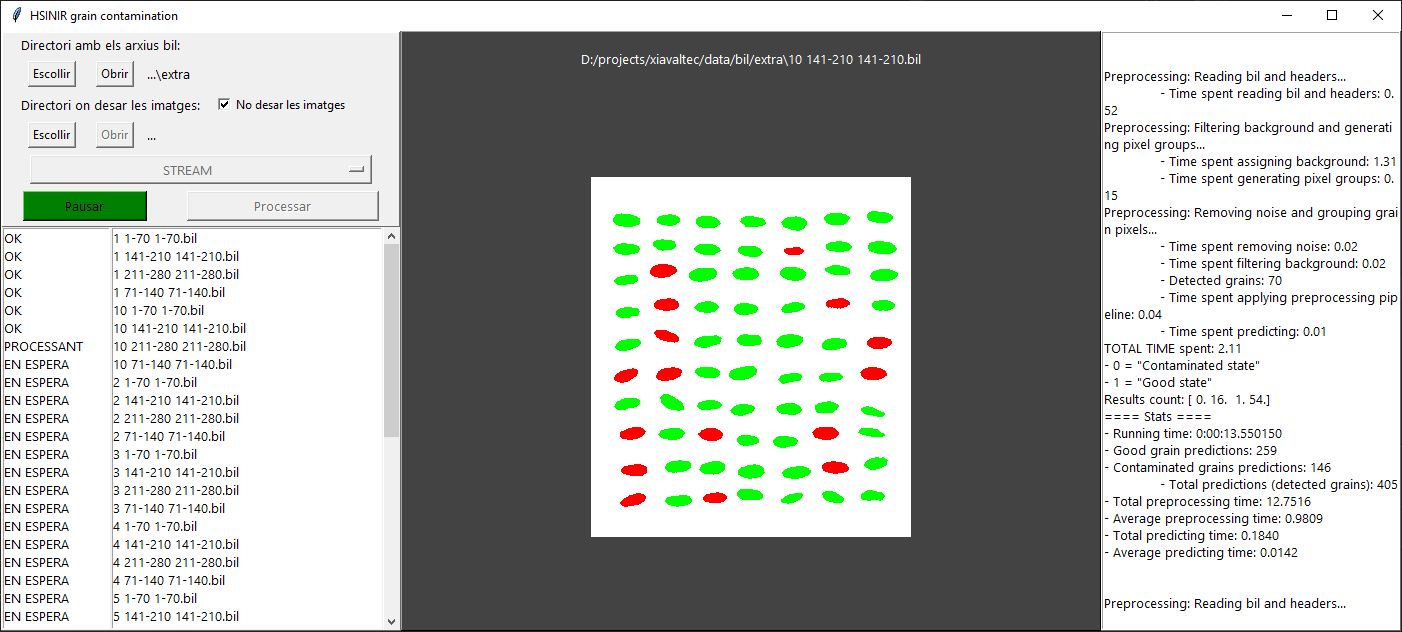
\includegraphics[width=0.8\textwidth]{media/images/example-execution-xiavaltec.png}
    \caption{Ejemplo de ejecución de la aplicación de escritorio. Fuente propia.}
    \label{fig:app-example}
\end{figure}

Aunque no sería la aplicación real, ya que esta debería estar conectada a un sistema de control, la aplicación de escritorio nos permite visualizar de forma sencilla los resultados de la predicción de contaminación de los granos.

\subsection{Comparación con el modelo estadístico}

Antes del entrenamiento de los diferentes modelos que hemos visto a lo largo del documento, existía un modelo estadístico que se utilizaba para predecir la contaminación de los granos. Ahora que hemos obtenido un nuevo modelo de predicción (\textit{RS K-Neighbors} de la \textit{Sección\ \ref{sec:hyperparameter-tuning-2}}), podemos comparar los resultados de ambos y decidir si hemos logrado una mejora en el proceso.
Para ello, hemos utilizado los datos del conjunto de \textit{test}, pues el modelo no ha entrenado con ellos y hemos comparado los resultados de las predicciones de ambos modelos sobre este. Los resultados de los modelos se pueden ver en la \textit{Figura\ \ref{fig:model-comparison}}, donde podemos ver que el modelo nuevo es mucho más preciso al detectar las muestras contaminadas como las sanas, podemos verlo en la diagonal principal de las matrices de confusión o en la \textit{Tabla\ \ref{tab:model-comparison-tab}}, donde se tiene en cuenta el balance del \gls{dataset}, habiendo una mejora de \textbf{44.415 (94.3\%)} sobre la \textit{balanced accuracy}.

\begin{figure}
    \centering
    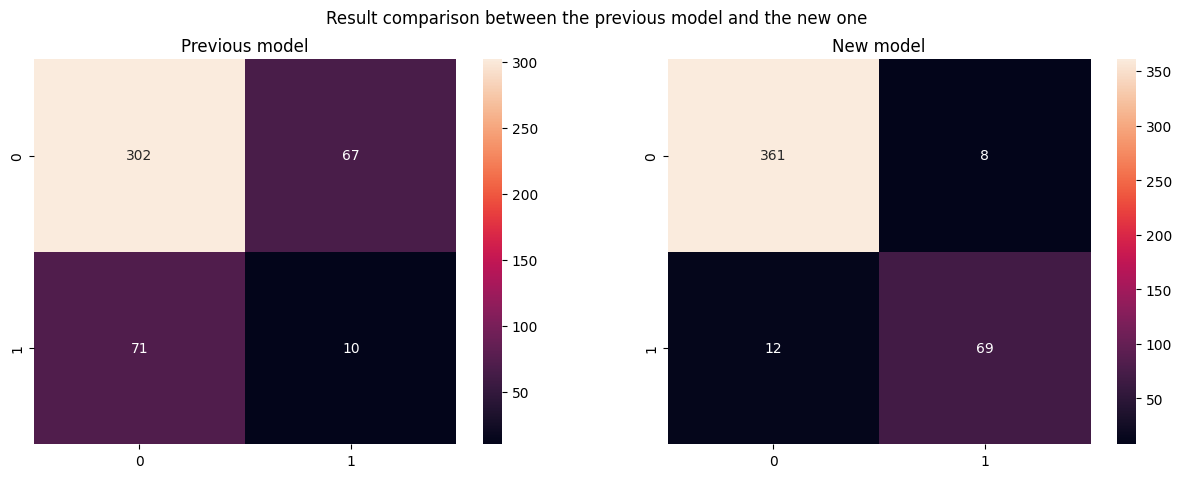
\includegraphics[width=\textwidth]{media/images/model-comparison.png}
    \caption{Comparación de los resultados de los modelos. Fuente propia.}
    \label{fig:model-comparison}
\end{figure}

\begin{table}
    \centering
    \begin{tabular}{|c|c|}
        \hline
        \textbf{Model} & \textbf{Balanced Accuracy} \\ \hline
        \textit{Modelo estadístico} & 47.094 \\ 
        \textit{\textbf{RS K-Neighbors}} & 91.509 \\ \hline
    \end{tabular}
    \caption{Resultados de los modelos sobre el dataset de prueba. Fuente propia.}\ \label{tab:model-comparison-tab}
\end{table}